\documentclass{article}
\usepackage[utf8]{inputenc}
\usepackage[]{thmtools}
\usepackage[]{xcolor}
\usepackage{graphicx}
\usepackage{hyperref}
\usepackage{lscape} 
\usepackage{amsmath}
\usepackage[]{cleveref}
\usepackage[]{geometry}
\geometry{textheight=10in}	
\usepackage{listings}
\usepackage{multirow}

\declaretheorem[shaded={rulecolor=gray}]{note} %shaded={rulecolor=gray}

\title{CMPUT 229 - RISC-V Green Sheet}
\author{andrew.miller5722 }
\date{January 2023}

\begin{document}
	\section{Week 1/2}
	\subsection{Introduction to RISC-V}
	\subsubsection{Binary Representation}
		All information passed through a processor can be expressed as a sequence of binary digits.
		
		Conversion between a base 2 number and a base 10 number can be done rather efficiently:\\
		\begin{equation}
			1001\,0111_2 = 151_{10}
		\end{equation}
	\begin{center}
		\begin{tabular}{c c c c}
			&1 & $\times 1$& 1\\
			&1 & $\times 2$& 2\\
			&1 & $\times 4$& 4\\
			&0 & $\times 8$& 0\\
			&&&\\
			&1 & $\times 16$& 16\\
			&0 & $\times 32$& 0\\
			&0 & $\times 64$& 0\\
			+&1 & $\times 128$& 128\\
			\hline
			& & & 151		 
		\end{tabular}
\end{center}
	\subsubsection{Hexadecimal Representation}
	We must also recall the hexadecimal representation of numbers that makes binary just a bit easier to look at. %todo, like the binary conversion to decimal
	\subsubsection{Two's Complement}
	This is a convention for the expression of signed numbers, such that the most significant bit is negative instead of positive.
	\begin{equation}
		1001\,0111 = -105_{10}
	\end{equation}
\begin{center}
\begin{tabular}{c c c c}
&1 & $\times 1$& 1\\
&1 & $\times 2$& 2\\
&1 & $\times 4$& 4\\
&0 & $\times 8$& 0\\
&&&\\
&1 & $\times 16$& 16\\
&0 & $\times 32$& 0\\
&0 & $\times 64$& 0\\
+&1 & $\times \textbf{-128}$& \textbf{-128}\\
\hline
& & & -105		 
\end{tabular}
\end{center}
\subsection{Data in Memory}
All elements in a computer's memory is labeled with a memory address and the units of data in a computer's memory is a byte, which is 8-bits and is represented (usually) as two hex characters $\verb|0xFF|_{16} = 1111\,1111_2 = 255_{10}$.

Each memory address is represented by a 4-byte word (32-bits) which are arranged sequentially for the given process

\begin{note}[Word]
	It should be remembered that the 32-bit piece of memory that we have is called a `word' in RISC-V 32 IF (which is the complete name of the instruction set we are dealing with). This is easy to remember since the processor acts on 32-bit instructions. More on this later. 
\end{note}
\begin{note}[Memory Allocation]
	Remember that the allocation of this memory is handled by the operating system, this is outside the scope of this class.
\end{note}
\subsection{Registers}
Registers are given a name in assembly, we will come back to this later and by now you already know about them.

They are just a whole bunch of faster-to-access storage locations for data and hold 1 word worth of data. %TODO don't do this to the reader
\subsubsection{Endian-ness}
RISC-V is little-endian, which means that we read the contents of memory from right to left. This is nice for the processor but not nice for us.

What little endian means is like this:
\begin{center}
	\begin{tabular}{ccccc}
		0x & 12 & 34 & 56 & 78\\
		&&&&$\uparrow$\\
	\end{tabular}
\end{center}
The byte with the arrow pointing to it is the first byte in the sequence, we then read to the left by \textbf{byte} (not bit). So, for example, if we stored the word `BEAN' into our 32-bit word, we would see this:
\begin{center}
\begin{tabular}{ccccc}
	0x & N & A & E & B\\
	&&&&$\uparrow$\\
\end{tabular}
\end{center}
If we were to represent the word in ASCII.
\begin{note}[ASCII Characters]
	The ASCII alphabet contains 256 characters, thus each ASCII character is represented in 1 byte (8 bits). \textbf{Excersize}, what is the binary representation for the 256th ASCII letter. 
\end{note}
If we take a look at the RISC-V Emulator, RARS, we can get a feel for a larger example of the little endian nature of riscv. %TODO

\subsection{Computer Organization}
\begin{figure}
	\begin{center}
		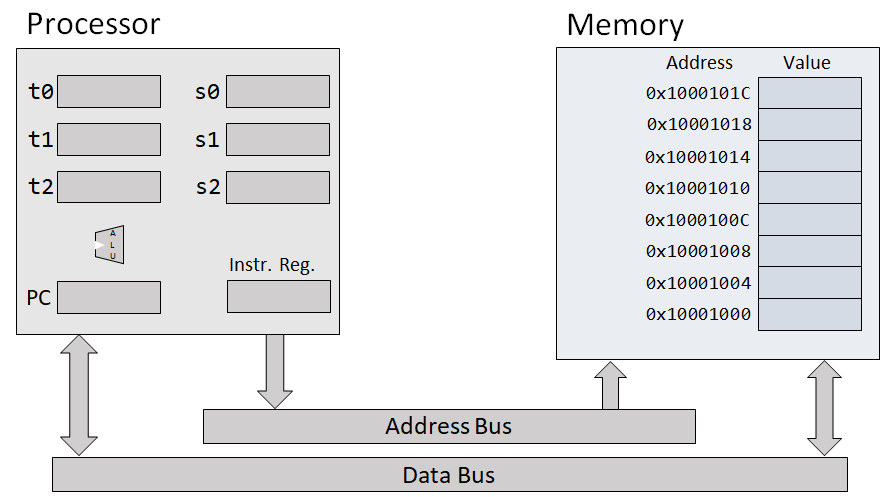
\includegraphics[scale=0.35]{cmporg.png}
	\end{center}
\caption[]{The organization of the processory and memory in a conventional computer detailing the contents of the processor registers and memory address-value map}
\label{fig:cmporg}
\end{figure}
\subsubsection{The Processor}
The processor is the brain of the computer and is used to perform the computations that we give it, we will learn more about the performance of the processor in the \ref{sec:perf} section. Some important things to note about the processor\footnote{These are mostly supplementary and begin diving into the nitty-gritty of how a processor is architected. I grabbed most of my information from \href[]{https://www.cs.umd.edu/~meesh/cmsc411/website/projects/outer/hoc/nontech.htm}{here}.}:
\begin{itemize}
	\item \textbf{Registers}: The fastest possible data access location.
	\item \textbf{I/D Cache}: The instruction and Data cache, they store information that is essentially ``currently in use'' (NEED VERIFICATION).
	\item \textbf{L0 cache}: Note that some computers do not have an L0 cache. This would be a cache to which the operational units have direct access. On the order of 128 bits wide.
	\item \textbf{L1 cache}: Typically the "on-chip split instruction and data caches" or "unified on-chip cache". These are fast caches that run at the chip clock speed and can be accessed within one cycle. Between 8kb and 32kb (lower case b is `bits').
	\item \textbf{L2 cache}: An external cache that is much larger (256kb to 2Mb) that can be accessed within some multiple of the CPU clock speed.
	\item \textbf{L3+ cache}: There can be many levels of cache, they generally get progressively slower and larger.
\end{itemize}
There are also some special registers in the processor that do important things:
\begin{itemize}
	\item \textbf{Instruction Register}: Keeps track of where we are in the program, more about this later. In RISC-V this is the program counter \verb|pc| register. %TODO link to the right section
	\item \textbf{Global Pointer}: %TODO
	\item \textbf{Return Address}: The address that stores the address to return to after an internal function call. More about this later. %TODO link
	\item \textbf{Stack Pointer}: The pointer to the base of the stack at the current moment. More about this later too. \verb|sp| %TODO link
	\item \textbf{Frame Pointer}: The pointer that points to the base of the current frame \verb|s0, fp|. This can double as another saved register in optimized code and is only ever used for debugging purposes.
	\item \textbf{Thread Pointer}: \verb|tp|%TODO
	\item \textbf{Temporary Registers}: \verb|t1 - t6|, for storing temporary data that can be erased at any point. Volatile registers.
	\item \textbf{Saved Registers}: \verb|s1 - s11|, for data that need to be preserved across function calls and exceptions.
\end{itemize}
\subsubsection{Memory}
This is essentially just a giant map of data with key-value pairs that represent certain data.

\subsubsection{Data Bus and Control Bus}
%TODO

\subsubsection{Storing and Loading from memory}
The two basic loading and storing operations in RISC-V are the \verb*|lw, sw| instructions which mean load-word and store-word respectively.%TODO


\section{Week 3}
\subsection{Instruction types and Immediates}
\subsubsection{Representing Instructions in Binary}
In order for a processor to understand what we want it to do, we need to convert our instructions into a binary format. Assembly language is one level abstracted from this binary representation and it is the job of the assembler to translate our code into a machine readable binary representation. Luckily for us, this translation is almost direct, so we can get to understand what is going on under the hood of the assembler.

There are some standard parts to the instructions that we need to recognize to fully understand what is happening:\footnote{This can be found on page 89 of (The Morgan Kaufmann Series in Computer Architecture and Design) David A. Patterson, John L. Hennessy - Computer Organization and Design RISC-V Edition, our class textbook.}
\begin{itemize}
	\item \textbf{opcode (7)}: The opcode gives the processor the first indication of what instruction we want it to perform.
	\item \textbf{func3 (3), func7 (7)}: The func3 and 7 parts along with the opcode specify exactly which instruction we are asking the process to do. The reason that these are placed apart (as you will see in the diagrams below) is because some types of instructions don't need the full func7 specifier and the splitting of these parts simplifies the development of the hardware. Additionally, extensions of the ISA support 16-bit instructions so the RISC-V architecture by default reads 16-bit chunks of data.
	\item \textbf{rd (5)}: The destination register, this is where the result of the register is stored if necessary.\footnote{You can really dive into this seperation thing, there si a presentation \href[]{https://inst.eecs.berkeley.edu//~cs61c/resources/su18_lec/Lecture7.pdf}{here} and a very good stack exchange answer \href[]{https://stackoverflow.com/questions/58414772/why-are-risc-v-s-b-and-u-j-instruction-types-encoded-in-this-way}{here} and a decent little debate with an insightful comment \href[]{https://stackoverflow.com/questions/42392369/why-are-opcode-field-and-funct-field-apart-in-mips}{here}}
	\item \textbf{rs1, rs2 (5)}: These are the argument registers. rs1 is the first one we type and rs 2 is the second, so in the command \lstinline[]|add t1, t2, t3|, \lstinline[]|t1| is r1 and so forth.5
\end{itemize}
\begin{landscape}
	%TODO transcribe the big diagrams into this document
	% Template
	%\begin{tabular}{|c|c|c|c|c|c|c|c|c|c|c|c|c|c|c|c|c|c|c|c|c|c|c|c|c|c|c|c|c|c|c|c|}
	%	\hline31&30&29&28&27&26&25&24&23&22&21&20&19&18&17&16&15&14&13&12&11&10&9&8&7&6&5&4&3&2&1&0\\
	%	\hline \multicolumn{7}{|c|}{funct7}&\multicolumn{5}{c|}{rs2}&\multicolumn{5}{c|}{rs1}&\multicolumn{3}{c|}{funct3}&\multicolumn{5}{c|}{rd}&\multicolumn{7}{c|}{opcode}\\
	%	\hline
	%\end{tabular}
	%%%%%%%%%%%%%%%%%% R-Type %%%%%%%%%%%%%%%%%%%%
	\begin{figure}
		\title{R-Type Instruction Representation}
		\begin{tabular}{|c|c|c|c|c|c|c|c|c|c|c|c|c|c|c|c|c|c|c|c|c|c|c|c|c|c|c|c|c|c|c|c|}
			\hline31&30&29&28&27&26&25&24&23&22&21&20&19&18&17&16&15&14&13&12&11&10&9&8&7&6&5&4&3&2&1&0\\
			\hline \multicolumn{7}{|c|}{funct7}&\multicolumn{5}{c|}{rs2}&\multicolumn{5}{c|}{rs1}&\multicolumn{3}{c|}{funct3}&\multicolumn{5}{c|}{rd}&\multicolumn{7}{c|}{opcode}\\
			\hline
		\end{tabular}
		\caption{R-Type instruction layout}
	\end{figure}
	%%%%%%%%%%%%%%%%%% I-Type %%%%%%%%%%%%%%%%%%%%
	\begin{figure}
		\title{I-Type Instruction Representation}
		\begin{tabular}{|c|c|c|c|c|c|c|c|c|c|c|c|c|c|c|c|c|c|c|c|c|c|c|c|c|c|c|c|c|c|c|c|}
			\hline31&30&29&28&27&26&25&24&23&22&21&20&19&18&17&16&15&14&13&12&11&10&9&8&7&6&5&4&3&2&1&0\\
			\hline s* &\multicolumn{11}{|c|}{imm[11:0]}&\multicolumn{5}{c|}{rs1}&\multicolumn{3}{c|}{funct3}&\multicolumn{5}{c|}{rd}&\multicolumn{7}{c|}{opcode}\\
			\hline
		\end{tabular}
		\caption{I-Type instruction layout, * the sign of the immediate, if loaded into a memory location, the immediate is sign extended down to bit 11 as shown in figure \cref{fig:imm_se}}
	\end{figure}
	%%%%%%%%%%%%%% Immediate Representation %%%%%%
	\begin{figure}
		\begin{tabular}{|c|c|c|c|c|c|c|c|c|c|c|c|c|c|c|c|c|c|c|c|c|c|c|c|c|c|c|c|c|c|c|c|}
			\hline31&30&29&28&27&26&25&24&23&22&21&20&19&18&17&16&15&14&13&12&11&10&9&8&7&6&5&4&3&2&1&0\\
			\hline \multicolumn{21}{|c}{sign} &\multicolumn{11}{|c|}{imm[11:0]}\\
			\hline
		\end{tabular}
		\caption[]{Representation of an 11-bit immediate in memory. Unsigned immediates are represented in the same way, simply adding one bit to the significant end.}
		\label{fig:imm_se}
	\end{figure}
	%%%%%%%%%%%%%%%%%% S-Type %%%%%%%%%%%%%%%%%%%%
	\begin{figure}
		\begin{tabular}{|c|c|c|c|c|c|c|c|c|c|c|c|c|c|c|c|c|c|c|c|c|c|c|c|c|c|c|c|c|c|c|c|}
			\hline31&30&29&28&27&26&25&24&23&22&21&20&19&18&17&16&15&14&13&12&11&10&9&8&7&6&5&4&3&2&1&0\\
			\hline s*&\multicolumn{6}{|c}{imm[11:5]} &\multicolumn{5}{|c|}{rs2}&\multicolumn{5}{|c|}{rs1}&\multicolumn{3}{|c|}{funct3}&\multicolumn{5}{|c|}{imm[4:0]}&\multicolumn{7}{|c|}{opcode}\\
			\hline
		\end{tabular}
		\caption[]{Representation of the S-Type instructions, note that the immediate is still 11 bits, it is simply split over two parts. Similarly to the I-type instructions, the immediate representation will follow the outlined form above.}
		\label{fig:instr-s}
	\end{figure}
	%%%%%%%%%%%%%%%%%% B-Type %%%%%%%%%%%%%%%%%%%%
	\begin{figure}
		\begin{tabular}{|c|c|c|c|c|c|c|c|c|c|c|c|c|c|c|c|c|c|c|c|c|c|c|c|c|c|c|c|c|c|c|c|}
			\hline31&30&29&28&27&26&25&24&23&22&21&20&19&18&17&16&15&14&13&12&11&10&9&8&7&6&5&4&3&2&1&0\\
			\hline s*&\multicolumn{6}{|c}{imm[10:5]} &\multicolumn{5}{|c|}{rs2}&\multicolumn{5}{|c|}{rs1}&\multicolumn{3}{|c|}{funct3}&\multicolumn{4}{|c|}{imm[4:1]}&[11]&\multicolumn{7}{|c|}{rs2}\\
			\hline
		\end{tabular}
		\caption[]{Representation of the S-Type instructions, note that the immediate in this case is 12 bits, and is again split over two parts. The reasoning behind this ordering can be found in chapter 4.4 of the textbook.}
		\label{fig:instr-b}
	\end{figure}
	%%%%%%%%%%%%%%%%%% U-Type %%%%%%%%%%%%%%%%%%%%
	\begin{figure}
		\title{Signed Immediate Representation}
		\begin{tabular}{|c|c|c|c|c|c|c|c|c|c|c|c|c|c|c|c|c|c|c|c|c|c|c|c|c|c|c|c|c|c|c|c|}
			\hline31&30&29&28&27&26&25&24&23&22&21&20&19&18&17&16&15&14&13&12&11&10&9&8&7&6&5&4&3&2&1&0\\
			\hline \multicolumn{20}{|c}{imm[31:12]} &\multicolumn{5}{|c|}{rd}&\multicolumn{7}{c|}{opcode}\\
			\hline
		\end{tabular}
		\caption[]{Representation of a U-Type instruction in binary.}
		\label{fig:instr-u}
	\end{figure}
\end{landscape}
\begin{tabular}{|c|c|c|c|c|c|c|c|}
	\hline\multirow{2}{*}{Name}&\multicolumn{6}{|c|}{Field}&\multirow{2}{*}{Comments}\\
	& 7 bits & 5 bits & 5 bits & 3 bits & 5 bits & 7 bits&\\
	\hline R-Type & funct7 & rs2 & rs1 & funct3 & rd & opcode & Arithmetic Instruction format\\
	\hline I-Type & \multicolumn{2}{|c|}{immediate[11:0]} & rs1 & funct3 & rd & opcode & Loads \& immediate arithmetic\\
	\hline S-Type & imm[11:5] & rs2 & rs1 & funct3 & imm[4:0] & opcode & Stores\\
	\hline SB-Type & imm[12, 10:5] & rs2 & rs1 & funct3 & imm[4:1,11] & opcode & Conditional Branch Statements\\
	\hline UJ-Type & \multicolumn{4}{|c|}{imm[20,10:1,11,19:12]} & rd & opcode & unconditional jump format\\
	\hline U-Type & \multicolumn{4}{|c|}{imm[31:12]} & rd & opcode & Upper immediate format\\ 
	\hline
\end{tabular}
\subsubsection{R-Type Instructions}
These are operations that work on multiple registers without any intermediates or interaction with memory, such as \verb|add,sub|.
\subsubsection{I-Type Instructions}
\subsubsection{S-Type  Instructions}
\subsubsection{B-Type  Instructions}
\subsubsection{U-Type  Instructions}
\subsubsection{JAL-Type  Instructions}
\subsection{Functions in RISC-V}
\section{Week 4}
\subsection{Performance}
\label{sec:perf}
Key formulae:
\begin{align}
	\text{Performance}_X&=\frac{1}{\text{Execution Time}}\\
	\text{CPI}&=\frac{\text{Clock periods}}{\text{Instructions}}\\
	\text{CPU Time} &=\frac{\text{Instruction count}\times\text{CPI}}{\text{Clock rate}}
\end{align}
\section{Week 5}
\subsection{Pointers}
\subsection{Computer Arithmetic}
\subsection{Locks}
\section{Week 6}
\subsection{Compiler Structure}
\subsection{Exceptions and Interrupts}
\subsection{I/O Devices}

\section{Appendices}
\subsection{Register Usages}
\begin{tabular}{|c|c|c|}
	\hline \textbf{Name} & \textbf{Number} & \textbf{Description}\\
	\hline ustatus & 0 &Interrupt status information (set the lowest bit to enable exceptions)\\
	\hline fflags &1&The accumulated floating point flags\\
	\hline frm    &2&Rounding mode for floating point operatations\\
	\hline fcsr   &3&Both frm and fflags\\
	\hline uie    &4&Finer control for which interrupts are enabled\\
	\hline utvec  &5&The base address of the interrupt handler\\
	\hline uscratch &64 & Scratch for processing inside the interrupt handler\\
	\hline uepc   &65&PC at the time the interrupt was triggered\\
	\hline ucause &66&Cause of the interrupt (top bit is interrupt vs trap)\\
	\hline utval  &67&Value associated with the cause\\
	\hline uip    &68&Shows if any interrupt is pending and what type\\
	\hline cycle  &3072&Number of clock cycles executed\\
	\hline time   &3073&Time since some time in the past (Milliseconds since 1/1/1970 in RARS)\\
	\hline instret&3074&Instructions retired (same as cycle in RARS)\\
	\hline cycleh &3200&High 32 bits of cycle\\
	\hline timeh  &3201&High 32 bits of time\\
	\hline instreth &3202&High 32 bits of instret\\\hline
\end{tabular}


\newpage 
\href[]{https://github.com/TheThirdOne/rars/wiki/Supported-Instructions}{Here} is a list of all the instructions supported by rars and the interpretation of those instructions.
\section{RISC-V Green Sheet (but better)}
\begin{tabular}{c|c|c|c|c|c}
		MNEMONIC & FMT & NAME & DESCRIPTION & NOTE & TYPE\\
		add, addi & \\
		and, andi
	\end{tabular}
	
	
\end{document}
